\ifx\boi\undefined\ifx\problemname\undefined
\providecommand\sampleinputname{}
\providecommand\sampleoutputname{}
\documentclass[lithuanian]{templates/boi}
\usepackage[L7x]{fontenc}
\problemlanguage{.lt}
\fi
\newcommand{\boi}{Baltijos šalių informatikos olimpiada}
\newcommand{\practicesession}{Bandomasis turas}
\newcommand{\contestdates}{2018 m. balandžio 27 - gegužės 1 d.}
\newcommand{\dayone}{1 diena}
\newcommand{\daytwo}{2 diena}
\newcommand{\licensingtext}{This problem is licensed under CC BY-SA 4.0.}
\newcommand{\problem}{Uždavinys}
\newcommand{\inputsection}{Pradiniai duomenys}
\newcommand{\outputsection}{Rezultatai}
\newcommand{\interactivity}{Realizacija}
\newcommand{\grading}{Vertinimas(?)}
\newcommand{\scoring}{Taškų skyrimas(?)}
\newcommand{\constraints}{Ribojimai}
\renewcommand{\sampleinputname}{Pradiniai duomenys}
\renewcommand{\sampleoutputname}{Rezultatai}
\newcommand{\sampleexplanation}[1]{Pirmojo pavyzdžio paaiškinimas}
\newcommand{\sampleexplanations}{Pavyzdžių paaiškinimai}
\newcommand{\timelimit}{Laiko ribojimas}
\newcommand{\memorylimit}{Atminties ribojimas}
\newcommand{\seconds}{s}
\newcommand{\megabytes}{MB}
\newcommand{\group}{Grupė}
\newcommand{\points}{Taškai}
\newcommand{\limitsname}{Ribojimai}
\newcommand{\additionalconstraints}{Papildomi ribojimai}
\newcommand{\testgroups}{
Jūsų sprendimas bus testuojamas su keliomis testų grupėmis, kiekviena kurių vertinama tam tikru skaičiumi taškų.
Kiekvieną testų grupę sudarys keletas testų.
Taškai už testų grupę skiriami tik jei įveikiate visus tos grupės testus.
}
\fi
\def\version{jury-1}
\problemname{Keliai}
{\em Grafas} -- matematinė struktūra, sudaryta iš {\em viršūnių} ir {\em briaunų} aibių, kur kiekviena briauna jungia dvi viršūnes. Grafo su $4$ viršūnėmis ir $3$ briaunomis pavyzdys pateiktas pavyzdinio testo paaiškinime.

{\em Kelias} apibrėžiamas kaip surikiuota $2$ ar daugiau viršūnių seka, tokia, kad bet kurias dvi gretimas sąrašo viršūnes jungia briauna. Šiame uždavinyje mus domina tik $paprastieji$ keliai, kuriuose jokia viršūnė nepasikartoja daugiau nei vieną kartą. Atkreipkite dėmesį, kad viršūnių tvarka kelyje yra svarbi -- pavyzdžiui, ``\texttt{5-6-7}'', ``\texttt{5-7-6}'' ir ``\texttt{7-6-5}'' yra laikomi skirtingais keliais.

Šiame uždavinyje kiekviena grafo viršūnė yra vienos iš galimų $K$ spalvų. Kiek yra tokių galimų (paprastųjų) kelių, kad visos konkrečiam keliui priklausančios viršūnės būtų skirtingų spalvų?




\section*{\inputsection}
Pirmoje eilutėje pateikiami trys sveikieji skaičiai: $N$ (viršūnių skaičius), $M$ (briaunų skaičius) ir $K$ (skirtingų spalvų skaičius).

%($1 \le N, M \le 3 \cdot 10^5, 1 \le K \le 5$).

Antroje eilutėje yra $N$ sveikųjų skaičių iš intervalo nuo $1$ iki $K$ -- visų viršūnių spalvos (pradedant $1$-ąja viršūne ir baigiant $N$-ąja). 

Tolimesnės $M$ eilučių nusako po briauną -- kiekvienoje pateikiama po du sveikuosius skaičius $a, b$ ($1 \le a, b \le N, a \neq b$) -- dvi briauna sujungtas viršūnes. Tarp bet kurių dviejų viršūnių bus ne daugiau nei viena briauna.

\section*{\outputsection}
Išveskite vieną sveikąjį skaičių -- skaičių kelių, kurių visos viršūnės yra skirtingų spalvų. Šis skaičius visada bus mažesnis nei $10^{18}$.

\section*{\constraints}
\testgroups

\noindent
\begin{tabular}{| l | l | l |}
\hline
\group & \points & \limitsname \\ \hline
1      & 23      & $1 \le N, M \le 100, 1 \le K \le 4$ \\ \hline
2      & 20      & $1 \le N, M \le 300\,000, 1 \le K \le 3$ \\ \hline
3      & 27      & $1 \le N, M \le 300\,000, 1 \le K \le 4$ \\ \hline
4      & 30      & $1 \le N, M \le 100\,000, 1 \le K \le 5$ \\ \hline
\end{tabular}

\section*{\sampleexplanation{1}}

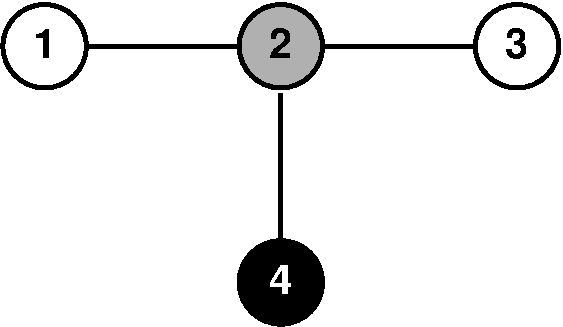
\includegraphics[width=5cm]{pathsfig.pdf}

Pirmojo sąlygos testo grafas pavaizduotas paveikslėlyje, kur visos viršūnės nuspalvintos baltai (spalva 1), pilkai (spalva 2) arba juodai (spalva 3). Yra 10 kelių, kuriuose visos viršūnės skirtingų spalvų: ``\texttt{1-2}'', ``\texttt{2-1}'', ``\texttt{2-3}'', ``\texttt{3-2}'', ``\texttt{2-4}'', ``\texttt{4-2}'', ``\texttt{1-2-4}'', ``\texttt{4-2-1}'', ``\texttt{3-2-4}'' ir ``\texttt{4-2-3}''.

Atkreipkite dėmesį, kad ``\texttt{1}'' nėra laikomas keliu, nes jame tik viena viršūnė, bei ``\texttt{1-2-3}'' neatitinka reikalavimų, nes turi dvi tos pčios spalvos ($1$) viršūnes.
